
\section[Individual parameter sensitivity]{Sensitivity Analysis of Individual Parameters near the Global Optimum}\label{sec:GA:IndividualSens}

\subsection{Individual Parameter Perturbation Analysis}\label{sec:GA:indiv-param-pert}

To further understand how useful each cost function was in
constraining parameters, a sensitivity analysis on each individual
parameter is is crucial to understand the behaviour of individual
parameters close to the global optimum.  The sensitivity analysis of
the cost function is defined as calculating the learning gradients of
each parameter on either side of the target value. Parameter values
were stepped up and down independently, with the steps determined from
the gene resolution of the parameter in
Table~\ref{tab:GA:Genome}. Gradients were calculated using a
least-squares linear regression in MATLAB/GNU Octave and two-sided
t-tests were performed to determine whether each gradient was
significantly different from zero.  This was done for the identical
and the different {\ANF} inputs, robustness was evaluated by comparing
the ratio of V-shaped to non-V-shaped cost function gradients for
different inputs.

\smallskip{}

Representative examples are given in Figure~\ref{fig:GA:R4}, which show
the dependence of the cost function on perturbation size when a
parameter was perturbed from its target value (and all other
parameters had their target value). A range of different behaviors is
evident depending on the particular combination of parameter and cost
function. The ideal behaviour is shown in Figure~\ref{fig:GA:R4}A, which
shows the target at a well defined local minimum in the cost function,
with significantly non-zero gradients bilaterally. Figure~\ref{fig:GA:R4}B is a sub-ideal case, with a significantly non-zero
gradient appearing only unilaterally, a zero gradient on the opposing
side.  The behaviour shown in Figure~\ref{fig:GA:R4}C, in which the cost
function is locally flat, implies that the cost function is
insensitive to this parameter in the vicinity of the target and
represents non-ideal behaviour. Finally, Figure~\ref{fig:GA:R4}D gives an
example of a problematic cost function behaviour, in which the minimum
occurs at a value other than the target.\yellownote{Hamish: I am
  still not happy we understand this well: Pruning of candidates with
  reduced spikes in low rate regions of DS units}. These cases were
classified variously as bilaterally sensitive (Figure~\ref{fig:GA:R4}A),
unilaterally sensitive (Figure~\ref{fig:GA:R4}B), insensitive (Figure~\ref{fig:GA:R4}C) or irregular(Figure~\ref{fig:GA:R4}D), respectively.
% Figure~\ref{fig:GA:12} shows four different examples of the individual
% parameter sensitivity for the ST cost function.  With the identical AN
% input, the ST cost function sensitivity to parameters 1 and 23
% ($w_{{\rm ANF}\to {\rm TS}} $ and $s_{{\rm DS}\to {\rm TV}} $) was
% significantly different from a flat gradient both above (Students'
% t-test p$<$0.0001) and below (p$<$0.0001) the target value.  When the
% {\ANF} input was slightly different from the ideal input, the optimum
% increases and the gradient of parameter 1, $w_{{\rm ANF}\to {\rm TS}}
% $, diminishes (Figure~\ref{fig:GA:12}C). The spread of connections from
% DS cells to TV cells is wide (target value=8 channels), covering one
% third of the network (30 channels) so the non-linear jumps could be
% due to random selection of pre-synaptic cells or confounding effects
% of TV cells on TS and DS cells. With different inputs, parameter 23
% ($s_{{\rm DS}\to {\rm TV}} $) sensitivity of the ST cost function was
% robust below the target but is negative above the target although not
% significantly. 
Gradients that oppose the direction toward the target
would reduce the effectiveness of optimization, especially
gradient-decent methods.  For parameters with a target value close to
the minimum range (parameters 17, 20, 26, and 27), the gradient below
the target were not considered in the sensitivity analysis.  Even with
identical {\ANF} inputs and the same random seed, a change in the number
of connections or spread parameters will alter the allocation of
synapses within the network.



% The gradients of the cost function above and below the target value are plotted
% in Figure ? for each individual parameter and for the three different cost
% functions. {\bf order and comment on similarities. Also comment on correlation
% between parameter sensitivity and parameter error.}
% 
% A summary of these data are given in Table ?, which compares the cost
% function on basis of how many parameters showed sensitivity that was
% bilateral, unilateral or absent, or contained opposing gradients.

% I would be better to present these results in table comparing



 \begin{figure}[tp!]
   \centering
   \includegraphics[width=\textwidth]{Example_SensAnalysis.eps}  
  \caption{Examples of ST cost function sensitivity analysis
    performed on individual parameters, with 10 unit step increments
    around the parameter's target value and all other target
    parameters retained. Multiple samples were taken at each point
    when different inputs were used. The linear regression line
    (solid) and bootstrapped 95\% confidence interval (dotted line)
    are shown. The slope was tested for significant difference to a
    zero gradient either side of the target value. (A) Parameter 3,
    $n_{{\rm HSR}\to {\rm TS}} $, was V-shaped for identical and
    different inputs. (B) Parameter 4, $w_{{\rm ANF}\to {\rm DS}} $,
    was V-shaped for identical inputs, but for different inputs the
    gradient below the target was significantly opposed to the
    correct direction. (C) Sensitivity around parameter 23, $s_{{\rm
        DS}\to {\rm TV}} $, was V-shaped for identical inputs but
    only one gradient was significant for different inputs. (D) The
    sensitivity of the ST cost function around parameter 29,
    $n_{{\rm GLG}\to {\rm DS}} $, produced the largest V-shaped
    gradients for identical and different inputs.}
  \label{fig:GA:R4}
\end{figure}

\subsubsection{Spike Timing}

The ST cost function showed sensitivity to 27 of the 30 parameters on
both sides of the target values with the identical {\ANF} input (Figure
13A), 2 parameters on one side and only one parameter 25 ($n_{{\rm
    TV}\to {\rm DS}} $) was completely insensitive. For different ANF
inputs (Figure~\ref{fig:GA:13}B), 11 parameters were bilaterally
sensitive and 8 were unilaterally sensitive, while the ST cost
function was completely insensitive to 6 parameters. Three parameters
controlling the excitatory synaptic input to DS cells, 4, 5 and 6
($w_{{\rm ANF}\to {\rm DS}} $, $n_{{\rm HSR}\to {\rm DS}} $, $n_{{\rm
    LSR}\to {\rm DS}} $) had significant opposing gradients below the
target, and the inhibitory input parameter 25 ($n_{{\rm TV}\to {\rm
    DS}} $) above the target suggesting a shifted optimum value.  DS
cells have very precise onset spikes and few spikes in the remainder
of the stimulus.  If the weight and number of excitatory inputs were
reduced, the spike timing difference would not be influence by (or
inhibitory input increased), the onset spikes would still occur but
the larger difference in the random positions the number of spikes in
the sustained period of the stimulus would be reduced and the there
would be some benefit to this change in the training data.

\smallskip{}

The synaptic parameters have a strong influence on the timing of
spikes in post-synaptic neurons, contributing to changes in the cost
function score when the parameters are moved further away from the
target, and provide a well-defined global optimum. Even though the
number of individual parameters with significant learning gradients
was reduced for the ST cost function with different inputs and there
were four parameters with significant opposing gradients (Figure 13B),
the cost function still produced a distinctive optimum (Figure 9B) and
the {\GA} was able to find genomes close to the global optimum.

\smallskip{}


% For different ANF
% inputs (Figure~\ref{fig:GA:13}B), 11 parameters were bilaterally
% sensitive and 8 were unilaterally sensitive, while the ST cost
% function was completely insensitive to 6 parameters. Three parameters
% controlling the excitatory synaptic input to DS cells, 4, 5 and 6
% ($w_{{\rm ANF}\to {\rm DS}} $, $n_{{\rm HSR}\to {\rm DS}} $, $n_{{\rm
% LSR}\to {\rm DS}} $) had significant opposing gradients below the
% target, and the inhibitory input parameter 25 ($n_{{\rm TV}\to {\rm
% DS}} $) above the target suggesting a shifted optimum value.

% When the {\ANF} input was slightly different from the ideal input, the optimum
% increases and the gradient of parameter 1, $w_{{\rm ANF}\to {\rm TS}}
% $, diminishes (Figure~\ref{fig:GA:12}C). The spread of connections from
% DS cells to TV cells is wide (target value=8 channels), covering one
% third of the network (30 channels) so the non-linear jumps could be
% due to random selection of pre-synaptic cells or confounding effects
% of TV cells on TS and DS cells. With different inputs, parameter 23
% ($s_{{\rm DS}\to {\rm TV}} $) sensitivity of the ST cost function was
% robust below the target but is negative above the target although not
% significantly. Gradients that oppose the direction toward the target
% would reduce the effectiveness of optimization, especially
% gradient-decent methods.  For parameters with a target value close to
% the minimum range (parameters 17, 20, 26, and 27), the gradient below
% the target were not considered in the sensitivity analysis.
% 
% DS cells have very precise onset spikes and few spikes in the remainder
% of the stimulus.  If the weight and number of excitatory inputs were
% reduced, the spike timing difference would not be influence by (or
% inhibitory input increased), the onset spikes would still occur but
% the larger difference in the random positions the number of spikes in
% the sustained period of the stimulus would be reduced and the there
% would be some benefit to this change in the training data.
% 


\begin{figure}[th]
  \centering
  \resizebox{\textwidth}{!}{%
    \includegraphics{STDYN_SensNormv2_Bar2.eps}%
    \includegraphics{STDYN_SensDiffv2_Bar2.eps}%
  }
  \caption{Parameter sensitivity gradient plots for the ST cost
    function with ideal input (A) and with different {ANF} input
    (B). Parameter gradients that are significantly different from
    zero (Student's t-test p $<$ 0.05) are shown with asterisk
    ($\ast$) and error bars that are the standard error of the
    slope. Gradients that are opposite to expected are shown in
    solid bars, with significant difference shown with a diamond
    ($\diamond$).}
  \label{fig:GA:13}
\end{figure}

\subsubsection{Instantaneous Firing Rate}

Figure~\ref{fig:GA:14} shows the individual parameter sensitivity of the
IFR cost functions.  The sensitivity of the IFR-25 cost function with
the identical inputs was significant for 54 of the possible 55
parameter gradients (Figure~\ref{fig:GA:14}A).  This matches the
well-defined global optimum of uniform parameter variation in
Figure~\ref{fig:GA:10}A.  The sensitivity to inhibitory parameters of the
IFR-25 cost function was not robust to changes in the {\ANF} input
(Figure~\ref{fig:GA:14}B) since most gradients were flattened (not
significant from zero gradient) or were unilaterally sensitive.  Seven
inhibitory parameters had opposing gradients below the target, but
only one was significant, 14 ($s_{{\rm DS}\to {\rm TS}} $). Parameter
10 had a significant reduction from identical inputs to different
inputs, where it became completely insensitive. %  The individual
% parameter sensitivity of the IFR-250 cost function with different
% inputs (Figure~\ref{fig:GA:14}C) is slightly changed from the IFR-25 cost
% function (14 opposing to insensitive, 8 and 10 insensitive to
% significant on one side, and 22 and 23 lost sensitivity on one side of
% the target).


% The sensitivity to inhibitory parameters of the
% IFR-25 cost function was not robust to changes in the {\ANF} input
% (Figure~\ref{fig:GA:14}B) since most gradients were flattened (not
% significant from zero gradient) or were unilaterally sensitive.  Seven
% inhibitory parameters had opposing gradients below the target, but
% only one was significant, 14 ($s_{{\rm DS}\to {\rm TS}} $). Parameter
% 10 had a significant reduction from identical inputs to different
% inputs, where it became completely insensitive.

\begin{figure}[th]
  \centering
  \resizebox{\textwidth}{!}{%
    \includegraphics{IFR25_SensNorm2_Bar2.eps}%
    \includegraphics{IFR25_SensDiffv2_Bar2.eps}%
  } 
 \caption{Parameter sensitivity gradient plots for the IFR cost function
    with the format similar to Figure~\ref{fig:GA:13}. (A) The IFR-25 cost
    function with identical input. (B) The IFR-25 cost function with
    different {ANF} inputs. %(C) The IFR-100 cost function with different ANF
%    inputs.
}
  \label{fig:GA:14}
\end{figure}


\subsubsection{Average Intracellular Voltage}

Figure~\ref{fig:GA:15}A shows the individual parameter sensitivity of the
AIV-25 cost function with identical inputs was similar to the IFR-25 cost
functions with 54 of the possible 55 parameters having significant
gradients.  The parameter sensitivity of the AIV-25 cost function was
reasonably robust to changes in the {\ANF} input despite a flattening of the
gradients (Figure~\ref{fig:GA:15}B), especially for excitatory parameters
(1-11). Thirteen parameters remained bilaterally sensitive parameters and 6
were unilaterally sensitive.  % The AIV-250 cost function also had flattened
% gradients with parameters 6, 10, 13 and 21 losing their significance to one
% side, while parameters 1 and 19 gained sensitivity to one side of the
% target (Figure~\ref{fig:GA:15}C).  Despite having the same range of cost
% function scores as the IFR cost function (between 0.15~and 0.5~sp/ms or
% mV), the mean of the AIV cost function's sensitivity gradients increased by
% a factor of 10.


\begin{figure}[ht]
  \centering
  \resizebox{\textwidth}{!}{%
    \includegraphics{IV25_SensNorm1_Bar2.eps}%
    \includegraphics{IV25_SensDiffv2_Bar2.eps}%
  }
  \caption{Parameter sensitivity gradient plots for the AIV cost
    function with the format similar to Figure~\ref{fig:GA:13}. A The
    AIV-25 cost function with identical input. (B) The AIV-25 cost
    function with different {ANF} inputs.% (C) The AIV-100 cost
%    function with different {\ANF} inputs.
}
  \label{fig:GA:15}
\end{figure}




\subsection[Correlation between sensitivity and best genome error]{Correlation between cost function sensitivity and GA best genome's parameter error}\label{sec:GA:corr-betw-sens}

\yellownote{Correlation between relative param error and gradient in Fig~\ref{fig:GA:BestGenomeVGradient} to be discussedfurther.  The LogLog results indicate a confirmation of our suspicion that the gradient would directly effect the eventual outcome of the best genomes. }

%\subsection{Best Genome Match to Individual Parameter Sensitivity}

\begin{figure}[th]
  \centering
  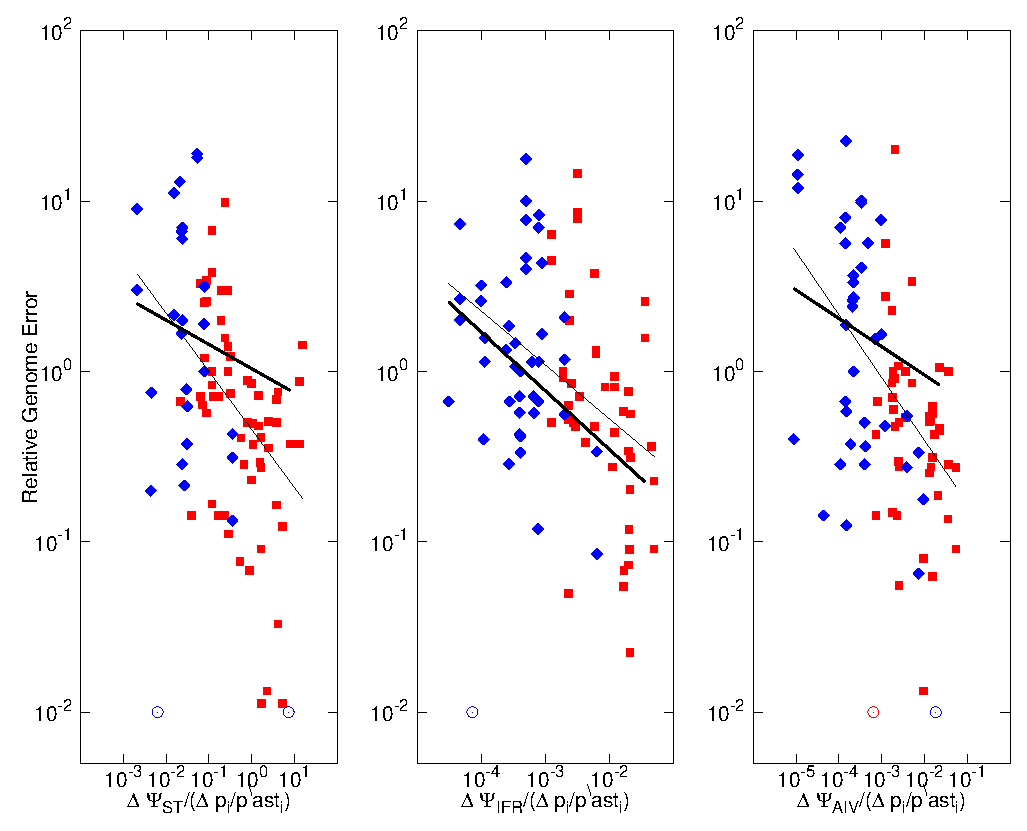
\includegraphics[width=\textwidth]{CombinedBestGenomeVSens-All}  
  \caption{Correlation of relative parameter error in {GA} best genomes
    against the sensitivity gradient of the training cost function
    (different {ANF} inputs, 25 repetitions). A Spike timing cost
    function (linear correlation p=0.0932 ,R$^2$=0.0317). B
    Instantaneous firing rate cost function (linear correlation
    p=0.0213 ,R$^2$=0.0588).  C Average intracellular voltage cost
    function (linear correlation p= 0.0144,R$^2$=0.0662).  More
    detailed analysis is available for each cost function in
    Tables~\ref{tab:GA:BGvGrad-ST}-\ref{tab:GA:BGvGrad-AIV}}
  \label{fig:GA:BestGenomeVGradient}
\end{figure}
% 

Regression of best genomes against the parameter gradients used the
function \textsf{regress} from GNU Octave's \textsf{statistics}
toolbox, which is a linear regression tool using least squares fit of
Y and X~\citep{Eaton:2002}. The significant level (alpha) used to
calculate the confidence interval was set to 0.05. The Y variable was
dependant on which side of the target the best genome's parameter lay
to determine the gradient; if there was no gradient (for targets too
close to the range termination), the other gradient was used. X was
the relative parameter error of the best genomes as used previously
($\left|p^\ast_i-{p}_i\right|/p^\ast_i$).

\smallskip{}

The regression analysis was performed for both linear and log-log
models. An additional test was done on data points restricted to those
whose cost function gradient passed the t-test in
section~\ref{sec:GA:indiv-param-pert}. For log-log regression, the
parameters with a perfect match (i.e.\ error of 0) were ignored due to
NaN elimination in the regression function.

\smallskip{}

\begin{table}[th]
  \centering
  \begin{tabular}{lccccc}
\toprule
                   &    m    & p-value  & R$^2$ &  F  & VAR(e) \\[1ex] \midrule
Linear (Pass Only) & -0.0623 &  0.286   & 0.0193& 1.16& 2.69   \\
LogLog (Pass Only) & -0.322  & 0.00284  & 0.141 & 9.7 & 0.338 \\[0.5ex] \hline
   Linear (All)    & -0.217  &  0.0932  & 0.0317& 2.88& 15     \\
   LogLog (All)    & -0.341  & 3.63e-06 & 0.217 & 24.4& 0.363 \\[1ex] \hline    
 \end{tabular}
 \caption{Best Genome vs.\ Gradient regression for ST cost function. $m$ is the gradient of the linear fit by least squares. $p$ is the p-value for the full model, where values  less than 0.05 indicate a significant fit of the model. $R^2$ is the sum of the residuals  squared, values above XXX show a good fit to the line.  F is the F-test statistic  indicating a sum of fit. VAR(e) is the estimated error variance.  }
  \label{tab:GA:BGvGrad-ST}
\end{table}


\begin{table}[th]
  \centering
  \begin{tabular}{lccccc}
                   &   m    & p-value  & R$^2$  &   F  & VAR(e) \\[1ex] \hline
Linear (Pass Only) & -59.1  &  0.0559  & 0.0824 & 3.86 & 7.25    \\
LogLog (Pass Only) & -0.583 & 0.00177  & 0.205  & 11.1 & 0.324  \\[0.5ex] \hline
   Linear (All)    & -65.4  &  0.0213  & 0.0588 & 5.5  & 9.13     \\
   LogLog (All)    & -0.317 & 1.65e-05 & 0.191  & 20.8 & 0.29   \\[1ex] \hline    
\end{tabular}
  \caption{Best Genome vs. Gradient regression for IFR cost function. See Table~\ref{tab:GA:BGvGrad-ST} for table explanation.}
  \label{tab:GA:BGvGrad-IFR}
\end{table}


\begin{table}[th]
  \centering
  \begin{tabular}{lccccc}
                   &   m    & p-value  & R$^2$  &  F   & VAR(e)\\[1ex] \hline
Linear (Pass Only) & -39.9  &  0.214   & 0.0327 & 3.86 & 7.25 \\
LogLog (Pass Only) & -0.344 &  0.0122  & 0.126  & 11.1 & 0.324\\[0.5ex] \hline
   Linear (All)    &  -101  &  0.0144  & 0.0662 & 5.5  & 9.13 \\
   LogLog (All)    & -0.368 & 1.81e-07 & 0.267  & 20.8 & 0.29 \\[1ex] \hline    
\end{tabular}
  \caption{Best Genome vs. Gradient regression for AIV cost function.  See Table~\ref{tab:GA:BGvGrad-ST} for table explanation.}
  \label{tab:GA:BGvGrad-AIV}
\end{table}


\yellownote{This paragraph has not been vetted.}

In summary, a log-log correlation has been observed between the each
of their cost function gradients near the target and the best genomes
trained with their cost function. Table~\ref{tab:GA:BGvGrad-ST} shows
a poor linear fit of the ST best genomes in
Figure~\ref{fig:GA:BestGenomeVGradient}, but a log-log model provides
a better fit, independent of the gradients' significance. This
behaviour was repeated for analysis of IFR
(Table~\ref{tab:GA:BGvGrad-IFR}) and AIV
(Table~\ref{tab:GA:BGvGrad-AIV}) best genomes; with the exception of
linear fit p-value of all AIV best genomes less than 0.05.  The few
perfect scores that were eliminated in the log-log regression
analysis, should not take away from the conclusion that the {\GAs}
eventual best genome relative error was directly log-correlated with
the cost function gradients around the target.


%%% Local Variables: 
%%% mode: latex
%%% TeX-master: "GAChapter"
%%% TeX-PDF-mode: nil
%%% End: 


